%%%%%%%%%%%%%%%%%%%%%%%%%%%%%%%%%%%%%%%%%
% Jacobs Landscape Poster
% LaTeX Template
% Version 1.1 (14/06/14)
%
% Created by:
% Computational Physics and Biophysics Group, Jacobs University
% https://teamwork.jacobs-university.de:8443/confluence/display/CoPandBiG/LaTeX+Poster
% 
% Further modified by:
% Nathaniel Johnston (nathaniel@njohnston.ca)
%
% This template has been downloaded from:
% http://www.LaTeXTemplates.com
%
% License:
% CC BY-NC-SA 3.0 (http://creativecommons.org/licenses/by-nc-sa/3.0/)
%
%%%%%%%%%%%%%%%%%%%%%%%%%%%%%%%%%%%%%%%%%

%----------------------------------------------------------------------------------------
%	PACKAGES AND OTHER DOCUMENT CONFIGURATIONS
%----------------------------------------------------------------------------------------

\documentclass[final,a0,portrait]{beamer}

\usepackage[scale=1.17]{beamerposter} % Use the beamerposter package for laying out the poster


\usetheme{confposter} % Use the confposter theme supplied with this template

\setbeamercolor{block title}{fg=ngreen,bg=white} % Colors of the block titles
\setbeamercolor{block body}{fg=black,bg=white} % Colors of the body of blocks
\setbeamercolor{block alerted title}{fg=white,bg=dblue!70} % Colors of the highlighted block titles
\setbeamercolor{block alerted body}{fg=black,bg=dblue!10} % Colors of the body of highlighted blocks
% Many more colors are available for use in beamerthemeconfposter.sty

%-----------------------------------------------------------
% Define the column widths and overall poster size
% To set effective sepwid, onecolwid and twocolwid values, first choose how many columns you want and how much separation you want between columns
% In this template, the separation width chosen is 0.024 of the paper width and a 4-column layout
% onecolwid should therefore be (1-(# of columns+1)*sepwid)/# of columns e.g. (1-(4+1)*0.024)/4 = 0.22
% Set twocolwid to be (2*onecolwid)+sepwid = 0.464
% Set threecolwid to be (3*onecolwid)+2*sepwid = 0.708

\newlength{\sepwid}
\newlength{\onecolwid}
\newlength{\twocolwid}
\newlength{\threecolwid}
%\setlength{\paperwidth}{48in} % A0 width: 46.8in
%\setlength{\paperheight}{36in} % A0 height: 33.1in
\setlength{\paperwidth}{86.1cm} % A0 width: 46.8in
\setlength{\paperheight}{118.9cm} % A0 height: 33.1in
\setlength{\sepwid}{0.01\paperwidth} % Separation width (white space) between columns
\setlength{\onecolwid}{0.3013\paperwidth} % Width of one column
\setlength{\twocolwid}{0.6026\paperwidth} % Width of two columns
\setlength{\threecolwid}{0.9040\paperwidth} % Width of three columns
\setlength{\topmargin}{-0.5in} % Reduce the top margin size
%-----------------------------------------------------------

\usepackage{graphicx}  % Required for including images
\graphicspath{{figures/}} % Directory in which figures are stored

\usepackage{booktabs} % Top and bottom rules for tables

%----------------------------------------------------------------------------------------
%	TITLE SECTION 
%----------------------------------------------------------------------------------------

\title{Designing a DORIS processing software for orbit determination and estimation of geodetic parameters} % Poster title
% \subtitle{}
\author{Xanthos Papanikolaou, Maria Tsakiri, Samuel Nahmani, Arnaud Pollet}% Author(s)

%\institute{Dionysos Satellite Observatory, School of Rural, Surveying \& Geoinformatics Engineering \\ \vspace{0.5em} \par{National Technical University of Athens}} % Institution(s)
\institute{Dionysos Satellite Observatory, School of Rural, Surveying \& Geoinformatics Engineering \\ \par{National Technical University of Athens}} % Institution(s)

%----------------------------------------------------------------------------------------

\begin{document}

\addtobeamertemplate{block end}{}{\vspace*{2ex}} % White space under blocks
\addtobeamertemplate{block alerted end}{}{\vspace*{2ex}} % White space under highlighted (alert) blocks

\setlength{\belowcaptionskip}{2ex} % White space under figures
\setlength\belowdisplayshortskip{2ex} % White space under equations

\begin{frame}[t] % The whole poster is enclosed in one beamer frame

\begin{columns}[t] % The whole poster consists of three major columns, the second of which is split into two columns twice - the [t] option aligns each column's content to the top

\begin{column}{\sepwid}\end{column} % Empty spacer column

\begin{column}{\onecolwid} % The first column

%----------------------------------------------------------------------------------------
%	INTRODUCTION
%----------------------------------------------------------------------------------------

\begin{block}{Introduction}
{\small
The \emph{Doppler Orbitography and Radiopositioning Integrated by Satellite} 
(DORIS) system was designed and developed by the French Space Agency CNES, jointly with 
the French National Geographic Institute (IGN) and the Research Group for Space 
Geodesy (GRGS). It is  based upon the accurate measurement of the Doppler shift 
of radio frequency signals transmitted from ground beacons and received on board 
the satellite. Its ground segment includes about 60 ground stations, equally 
distributed over the Earth and ensure a good coverage for orbit determination.

Dionysos Satellite Observatory (DSO) of the National Technical University of 
Athens (NTUA) has been hosting a \emph{Doppler Orbitography and Radiopositioning 
Integrated by Satellite} (DORIS) beacon since 1989, named \texttt{DIONYSOS/DIOB} 
\ref{fig:dionysos-beacon}. Since 2021, DSO has made the decision to expand its 
contribution to the DORIS community by developing its own, in-house processing 
software for precise orbit determination and positioning using the DORIS system.
%Currently, we have focused our efforts in reprocessing all the available GNSS data up to date, via Bernese GNSS Software v5.2\cite{bernese}.
}

\begin{figure}
\begin{tikzpicture}
  \node (img1) {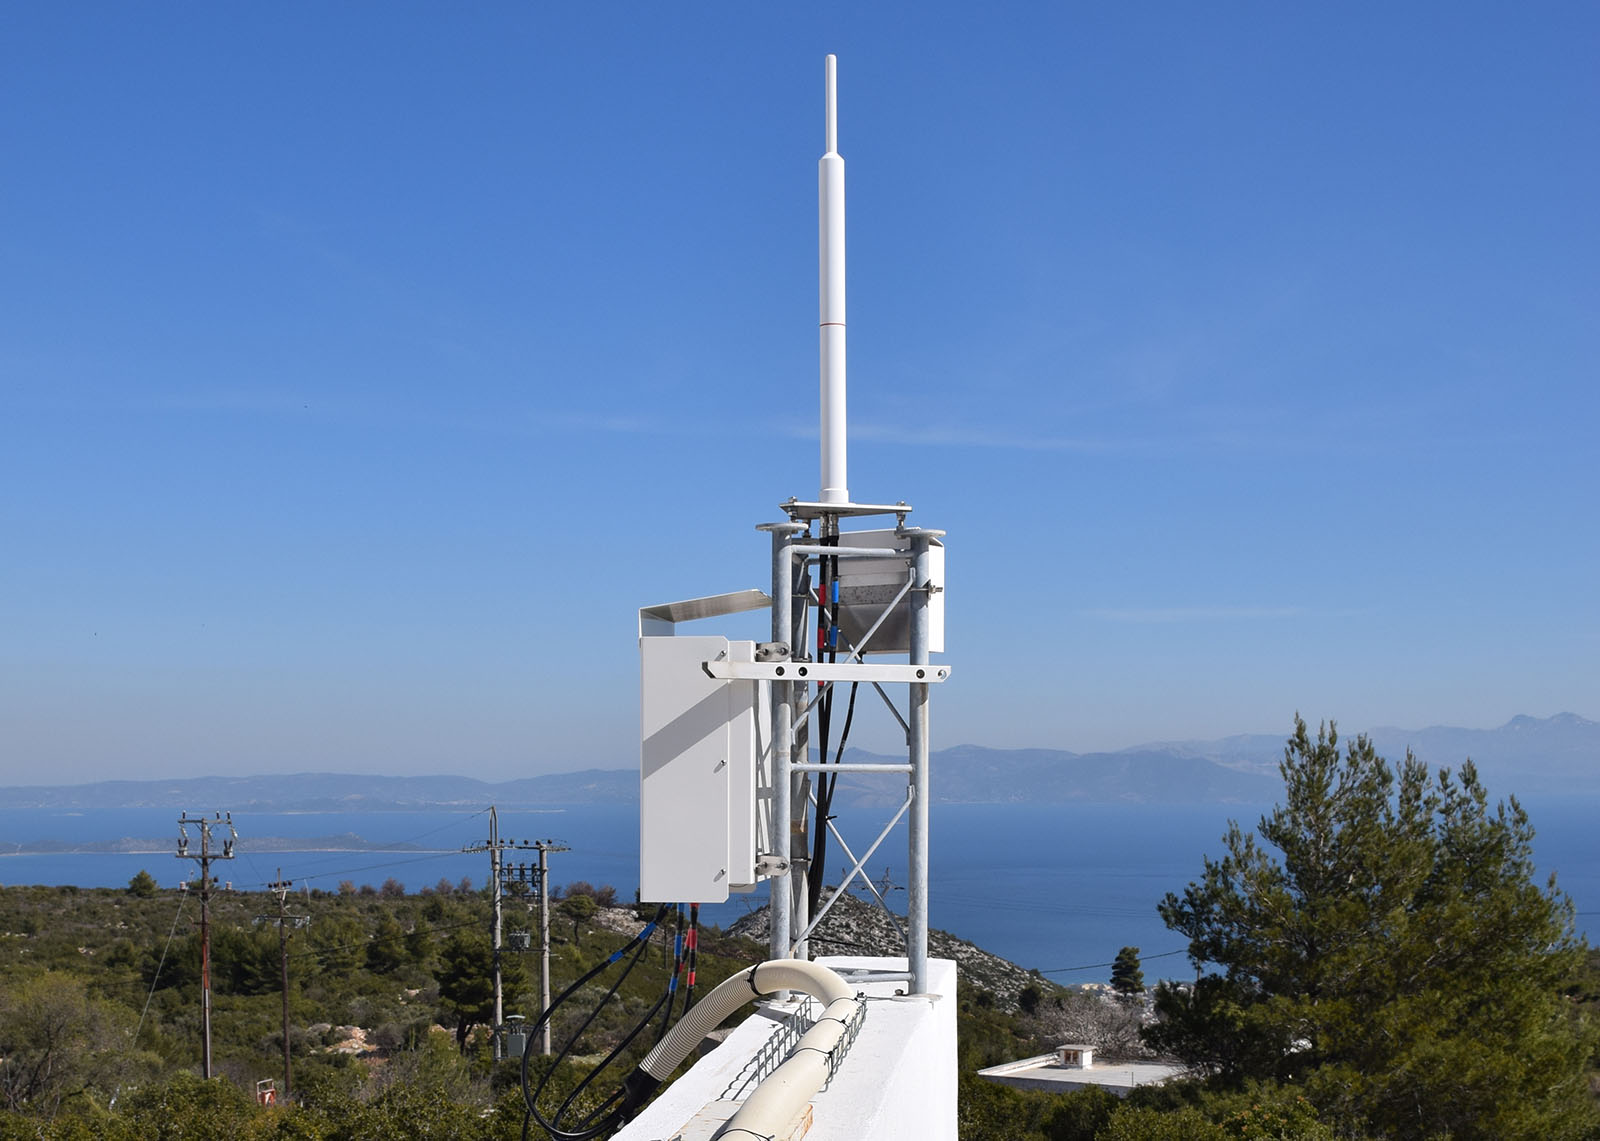
\includegraphics[width=0.7\onecolwid]{DIOB_202103}};
  \pause
  \node (img2) at (img1.east) {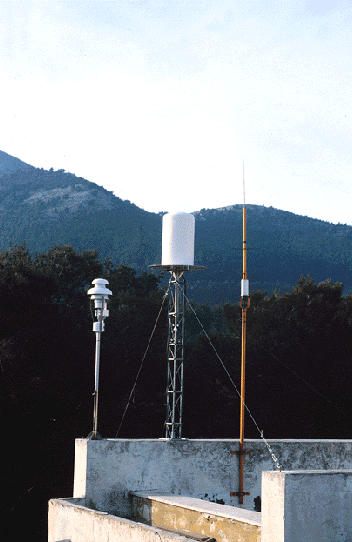
\includegraphics[width=0.4\onecolwid]{DIOA}};
\end{tikzpicture}
  \caption{\texttt{DIONYSOS} DORIS beacon installed at DSO. First installed 
  \texttt{DIOA} on the right, and the upgraded \texttt{DIOB} beacon on the 
  left.}
  \label{fig:dionysos-beacon}
\end{figure}

\end{block}
%------------------------------------------------
%           DATA
%------------------------------------------------
\begin{block}{Software Design}
{\small
Core software development will be performed using the \texttt{C++} programming 
language, taking advantage of its speed and versatility. Various minor, 
peripheral parts of the package will be developed using \texttt{Python}, 
allowing development speed and ease of use (for end users).

The software is being developed in an ``open'' fashion, using public 
repositories on \texttt{github}. Our intention is for the resulting software 
to be free of charge and open-source, so that the community can benefit as 
much as possible.

At a first step, we are targeting the \emph{Joint Altimetry Satellite 
Oceanography Network–3} (Jason-3) mission, using measured satellite attitude 
(quaternion approach).

Modeling is based on the current Internation DORIS Service (IDS, \cite{10.1007/1345_2015_164} ) recomendations 
for ITRF 2020 reprocessing (\cite{ids-itrf2020-recommendations}) and the 
International Earth Rotation Service (IERS) standards (\cite{iers2010}).
}
%\begin{figure}
%  \centering
%  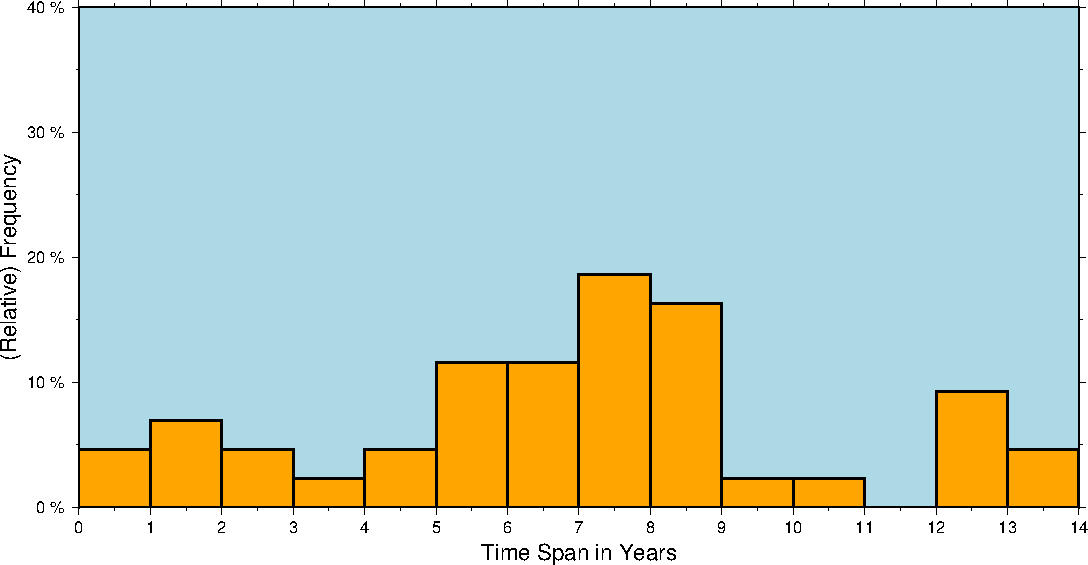
\includegraphics[width=1\onecolwid]{sample}
%  \caption{GNSS stations prosseced at DSO.}
%  \label{fig:sta}
%\end{figure}
\end{block}

%\bigskip
%\begin{alertblock}{Contact Information}
%\begin{itemize}
%\item Web: \href{http://dionysos.survey.ntua.gr}{dionysos.survey.ntua.gr}
%\item Email: \href{xanthos@mail.ntua.gr}{xanthos@mail.ntua.gr}
%\end{itemize}
%\end{alertblock}

%----------------------------------------------------------------------------
%	CONTACT INFORMATION
%----------------------------------------------------------------------------

%\setbeamercolor{block alerted title}{fg=black,bg=norange} % Change the alert block title colors
%\setbeamercolor{block alerted body}{fg=black,bg=white} % Change the alert block body colors
\textbf{Acknowledgments}
\par\textit{\footnotesize This project was funded by the National Technical 
University of Athens (NTUA), via its Program for Basic Research (PEVE 2021), 
within the framework of the \emph{Integrated Tropospheric Estimation in DORIS 
Satellite Positioning} (INESTRO, 65/2321) project.}

\par\textit{\footnotesize The authors would like to thank the International DORIS 
Service for making data and technical resources publicly available. We would also 
like to thank IDS members and especially Mr. Guilhem Moreaux for providing 
feedback and information.}

\begin{alertblock}{Contact Information}
\begin{itemize}
\item Web: \href{http://dionysos.survey.ntua.gr}{dionysos.survey.ntua.gr}
\item Email: \href{xanthos@mail.ntua.gr}{xanthos@mail.ntua.gr}
\end{itemize}
\end{alertblock}



%-----------------------------------------------------------------------------

\end{column} % End of the first column
%\vrule{}

% Empty spacer column
\begin{column}{\sepwid}\end{column}

% Begin a column which is two columns wide (column 2)
\begin{column}{\onecolwid} 

%--------------------------------------------------------------------------
%	PROCESSING
%---------------------------------------------------------------------------

\begin{block}{Processing \& Analysis}

{\small
DORIS data are extracted using the \texttt{RINEX DORIS 3.0} format 
(\cite{DORISRNX3}). Observation equations are formed following the approach 
outlined in \cite{lemoine-2016}:

\begin{subequations} \label{eq:lem13}
    \begin{align}
        v_{measured} & = \frac{c}{f_{e_N}} (f_{e_N} - f_{r_T} -
          \frac{N_{DOP}}{\Delta\tau_r}) + \Delta v_{REL} + 
          \Delta v_{IONO} \label{eq:lem13a} \\
        v_{theo} &= \frac{\rho_2 - \rho_1}{\Delta\tau_r} +
          \Delta v_{TROPO} - \frac{c(\frac{N_{DOP}}{\Delta\tau_r} + 
          f_{r_T})}{f_{e_N}} \frac{\Delta f_e}{f_{e_N}} \label{eq:lem13b}
    \end{align}
\end{subequations}

where:

\begin{description}
  \item $_{e_N}$ is ``nominal'' frequency of the emmiter ($2GHz$),
%
  \item $N_{DOP}$ is the \emph{Doppler count}, i.e. the difference between two 
  phase measurements done at different time tags, in the proper time scale of 
  the receiver (at the $2GHz$ carrier),
%
  \item $f_{r_T}$ is the ``true'' proper frequency of the receiver, obtained 
  using the respective \texttt{RINEX} file, after performing a one-day linear 
  smoothing,
%
  \item $\frac{\Delta f_e}{f_{e_N}}$ is the relative frequency offset for the 
  emmiter, accounting for differences between the nominal and true frequencies,
%
  \item $\Delta v_{REL} = \frac{1}{c} \left[ U_{r} - U_{e} + \frac{V^2_r - V^2_e}{2} \right]$ is computed using the $J_2$ contribution (\cite{lemoine-2016}),
%
  \item $\Delta v_{IONO}$ is the ionospheric correction, computed after 
  converting to iono-free phase measurement on the $2GHz$ channel, via 
  (\cite{lemoine-2016}):
  \begin{equation}
    \begin{aligned}
      L_{iono-free-2GHz} &= \frac{\gamma L_{2GHz} -
          \sqrt{\gamma}L_{400MHz}}{\gamma - 1} \\
                     &= L_{2GHz} + \frac{L_{2GHz} -
                        \sqrt{\gamma}L_{400MHz}}{\gamma - 1}
    \end{aligned}
  \end{equation}
  and applying respective reductions for the beacon and satellite phase centers, 
  using $\vec{r}_{iono-free-2GHz} = \frac{\vec{r}_{400MHz,2GHz}}{\gamma - 1}$

  \item $\Delta v_{TROPO}$ accounts for the correction due to the signal's travel 
  through the troposphere. For tropospheric path delay modeling, we use the 
  well established formula:
  \begin{equation}
    \Delta _{trop} = L_{z}^{hyd} \cdot mf_{el}^{hyd} + L_{z}^{wet} \cdot mf_{el}^{wet}
  \end{equation}
  where $L_{z}$ is the zenith path delay and $mf_{el}$ are the mapping functions 
  for the wet and hydrostatic parts respectively. We use the \texttt{GPT3/VMF3} 
  (\cite{Landskron2018}) to compute atmospheric parameters and $mf_{el}^{hyd}$ 
  values.

\end{description}

$\frac{\Delta f_e}{f_{e_N}}$ and $mf_{el}^{wet}$ are estimated during the 
processing, per beacon and satellite pass; for the former, we use a linear 
model approach. \hfill \break

Parameter estimation is performed via the \emph{Extended Kalman Filter} 
(e.g. \cite{ZHOU20201700}) algorithm, in ``one-pass'' mode, determining 
values for the satellite state, beacon-specific and orbital parameters 
(atmospheric drag and solar radiation pressure coefficients). \hfill \break

An elevation-dependent data (down)weighting scheme is followed, using the 
formula $1 / \sin (el)$. We use the RINEX-derived measurement flags to perform 
a basic data screening of the observations, complemented by a running 
$3\sigma$ test. \hfill \break

We follow the ``Variational Equations'' approach to perform orbit integration, 
solving for the initial value (ODE) problem using a slightly altered form of 
the algorithm described in \cite{alma992703343902959}. \hfill \break

We have chosen to use the \texttt{RINEX DORIS 3.0} format, to 
\begin{itemize}
  \item enable use of all modern features the format allows,
  \item enable use of carrier-phase measurements (later on),
  \item enable use of near real-time data files
\end{itemize}
}

%\begin{figure}
%  \centering
%  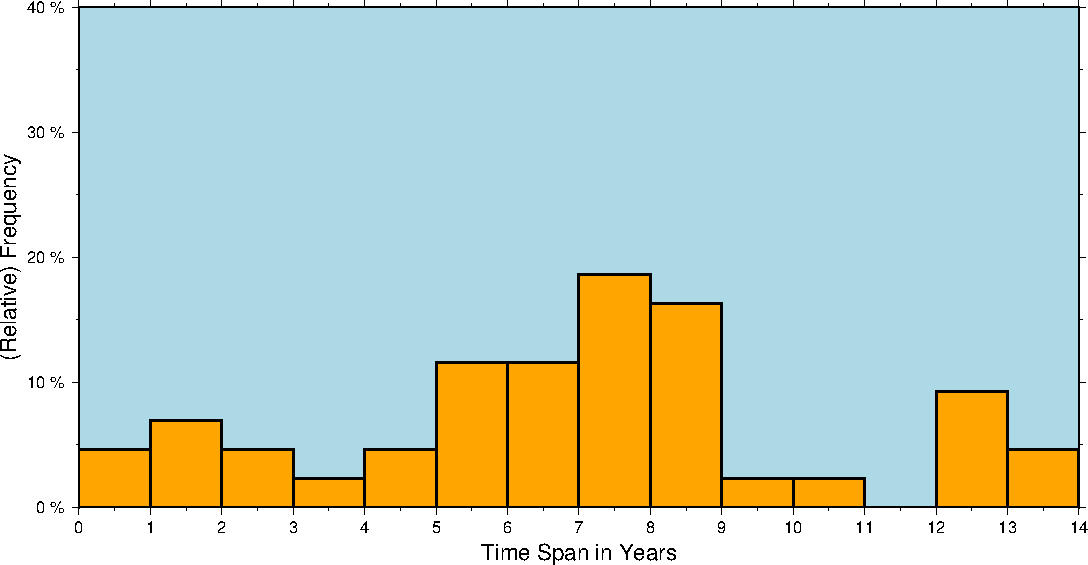
\includegraphics[width=0.7\onecolwid]{sample}
%  \caption{Flowchart of processing work.}
%  \label{fig:proc}
%\end{figure}
\end{block}

%-------------------------------------------------------------------------
%	PRELIMINARY RESULTS
%-------------------------------------------------------------------------

%\begin{block}{Preliminary Results}
%{\small
%Time series analysis follows an iterative process, where at each step one and/or more new parameters are tested based on their statistical significance.
%
%Tectonic velocities were estimated and the velocity field was produced, with respect to IGb2014 for stations with data availability greater than 2.5 years. A velocity field with respect to a stable Europe was estimated (Figure \ref{fig:crvels}) using the model Kreemer et al.(2014)\cite{kreemer14}.
%
%The StrainTool software is used with minor modifications \cite{straintool}, to estimate strian rates (Figure \ref{fig:strain}), dilatation (Figure \ref{fig:dil}) and the other parameters of the strain tensor on a grid with 0.25 deg. grid step.
%
%\begin{figure}
%  \centering
%  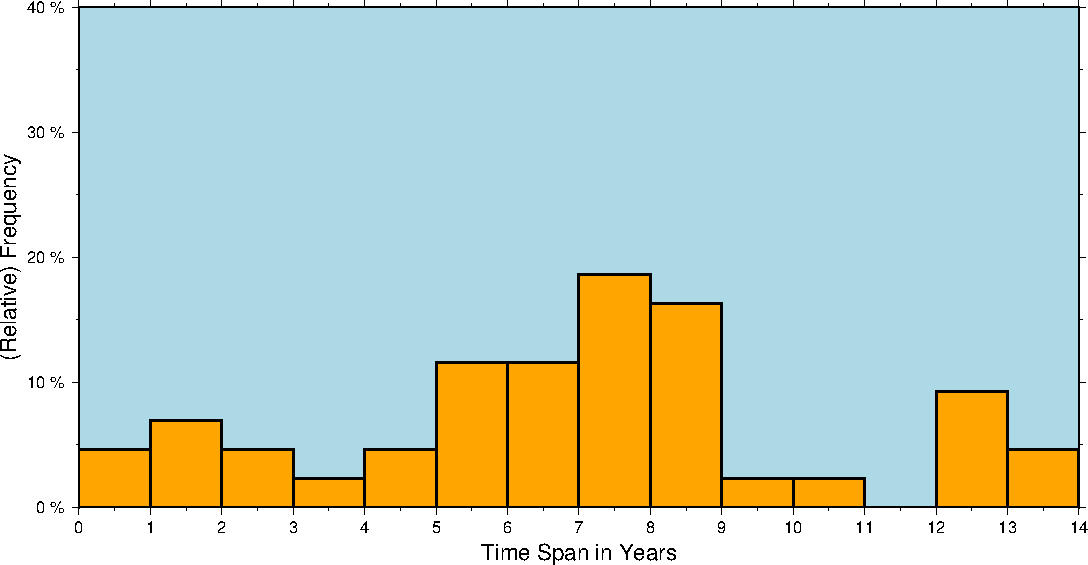
\includegraphics[width=1\onecolwid]{sample}
%  \caption{Velocity field}
%  \label{fig:crvels}
%%\end{minipage}
%\end{figure}
%
%\begin{figure}
%\centering
%\begin{minipage}{.5\textwidth}
%    \centering
%    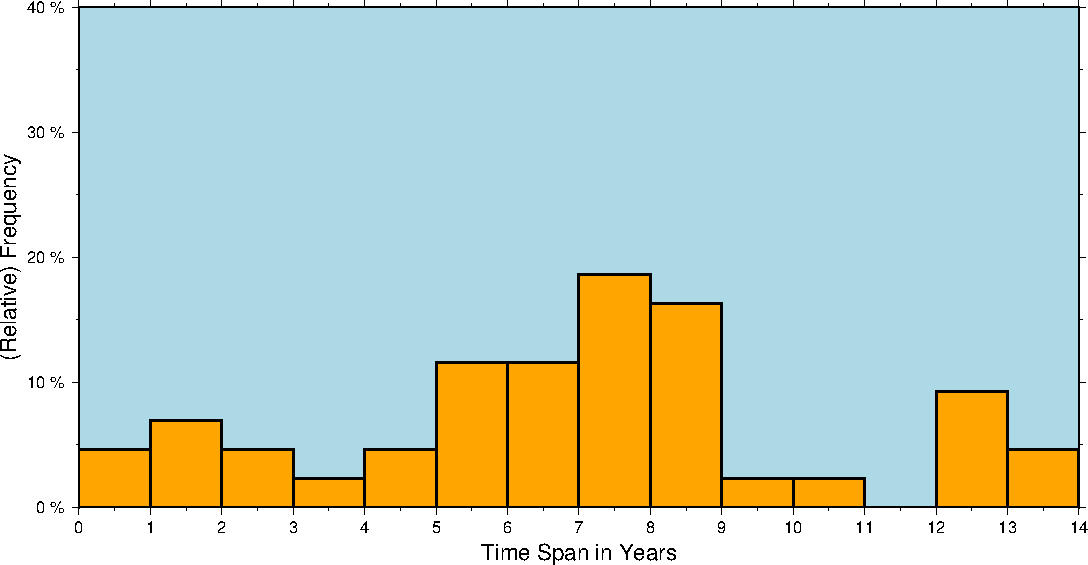
\includegraphics[width=1\linewidth]{sample}
%    %\captionof{figure}{A figure}
%    \caption{Strain rates} %%\url{http://dionysos.survey.ntua.gr/dsoportal/_projects/IonoRemSens/}.}
%    \label{fig:strain}
%\end{minipage}%
%\begin{minipage}{.5\textwidth}
%    \centering
%    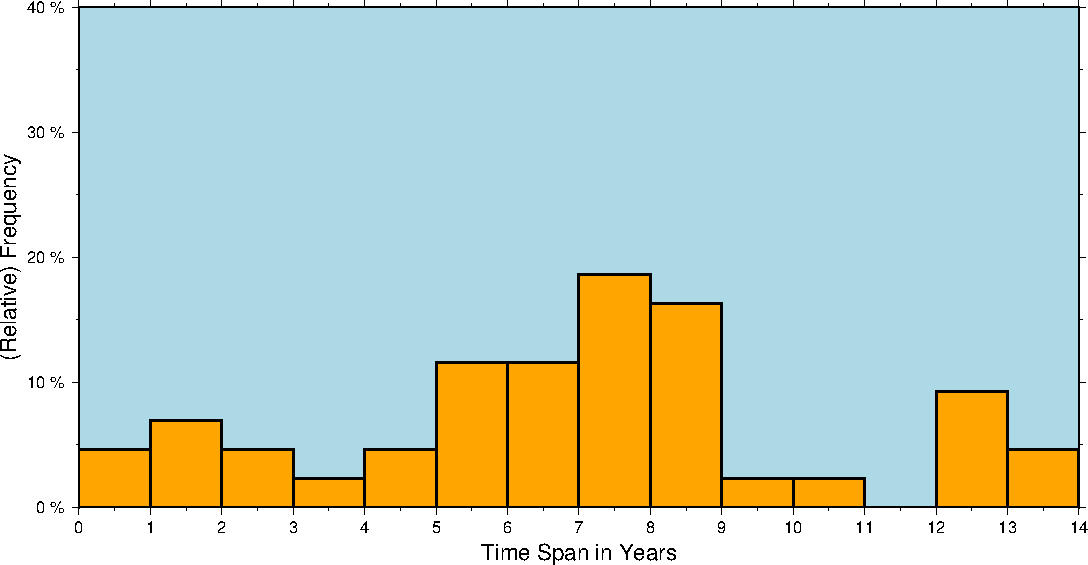
\includegraphics[width=1\linewidth]{sample}
%    %\captionof{figure}{Another figure}
%    \caption{Dilatation.}
%    \label{fig:dil}
%\end{minipage}
%\end{figure}
%
%
%}
%\end{block}

%----------------------------------------------------------------------------------------

\end{column} % End of the second column

\begin{column}{\sepwid}\end{column} % Empty spacer column

%\vrule{}

\begin{column}{\onecolwid} % The third column

%----------------------------------------------------------------------------------------
%	ONLINE PLATFORM
%----------------------------------------------------------------------------------------

\begin{block}{Online Platform}
{\small
The development of the website has been carried out with the programming tool (web framework) Django (djangoproject.com). At the same time, different parts of the website require the development of code in javascript, html and css, mainly for the visualization and formatting of the page. The platform is accessible at \url{http://dionysos.survey.ntua.gr/dso/enceladus/} 

The website presents the permanent GNSS stations whose data is available for processing by all networks.

A dynamic page is created for each station that participates in the monitoring of the Gulf of Corinth. Each page includes the station's data and all the necessary hyperlinks so that the user can access the processing products and the results.

For each solution day, at the end of the processing, the time series of the station is updated and the corresponding parameters obtained after the analysis of the position time series are given (Figure \ref{fig:vels}).

Finally, separate sections of the platform have been developed where the velocity fields and the estimation of the strain tensors are presented.

}

%\begin{figure}
%    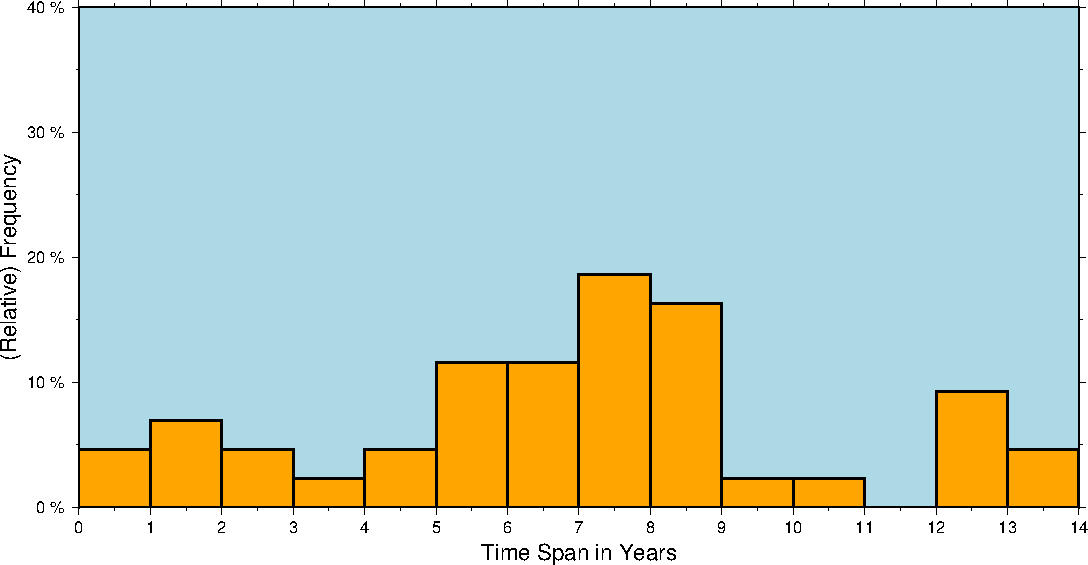
\includegraphics[width=1\onecolwid]{sample}
%    \caption{Times series analysis on platform.}
%    \label{fig:vels}
%\end{figure}

\end{block}

%----------------------------------------------------------------------------------------
%	CONCLUSION
%----------------------------------------------------------------------------------------


\begin{block}{Conclusion}
{\small
The main purpose of the project was to utilize all available GNSS data solution for the Corinthian Gulf region, to estimate the kinematic behavior.
The use of a large number of stations installed in the area has created a dense network that is analyzed daily.
A reliable velocity field has been produced from the time series analysis analysis, while correspondingly a primary strain field has been estimated.
The online platform, connected to the website of the EnCeldus Supersite, is the hub for the distribution of the results of the analysis for all the available data. The scientific community can use the platform to enhance the research in different scientific fields.

}
% \begin{figure}
%     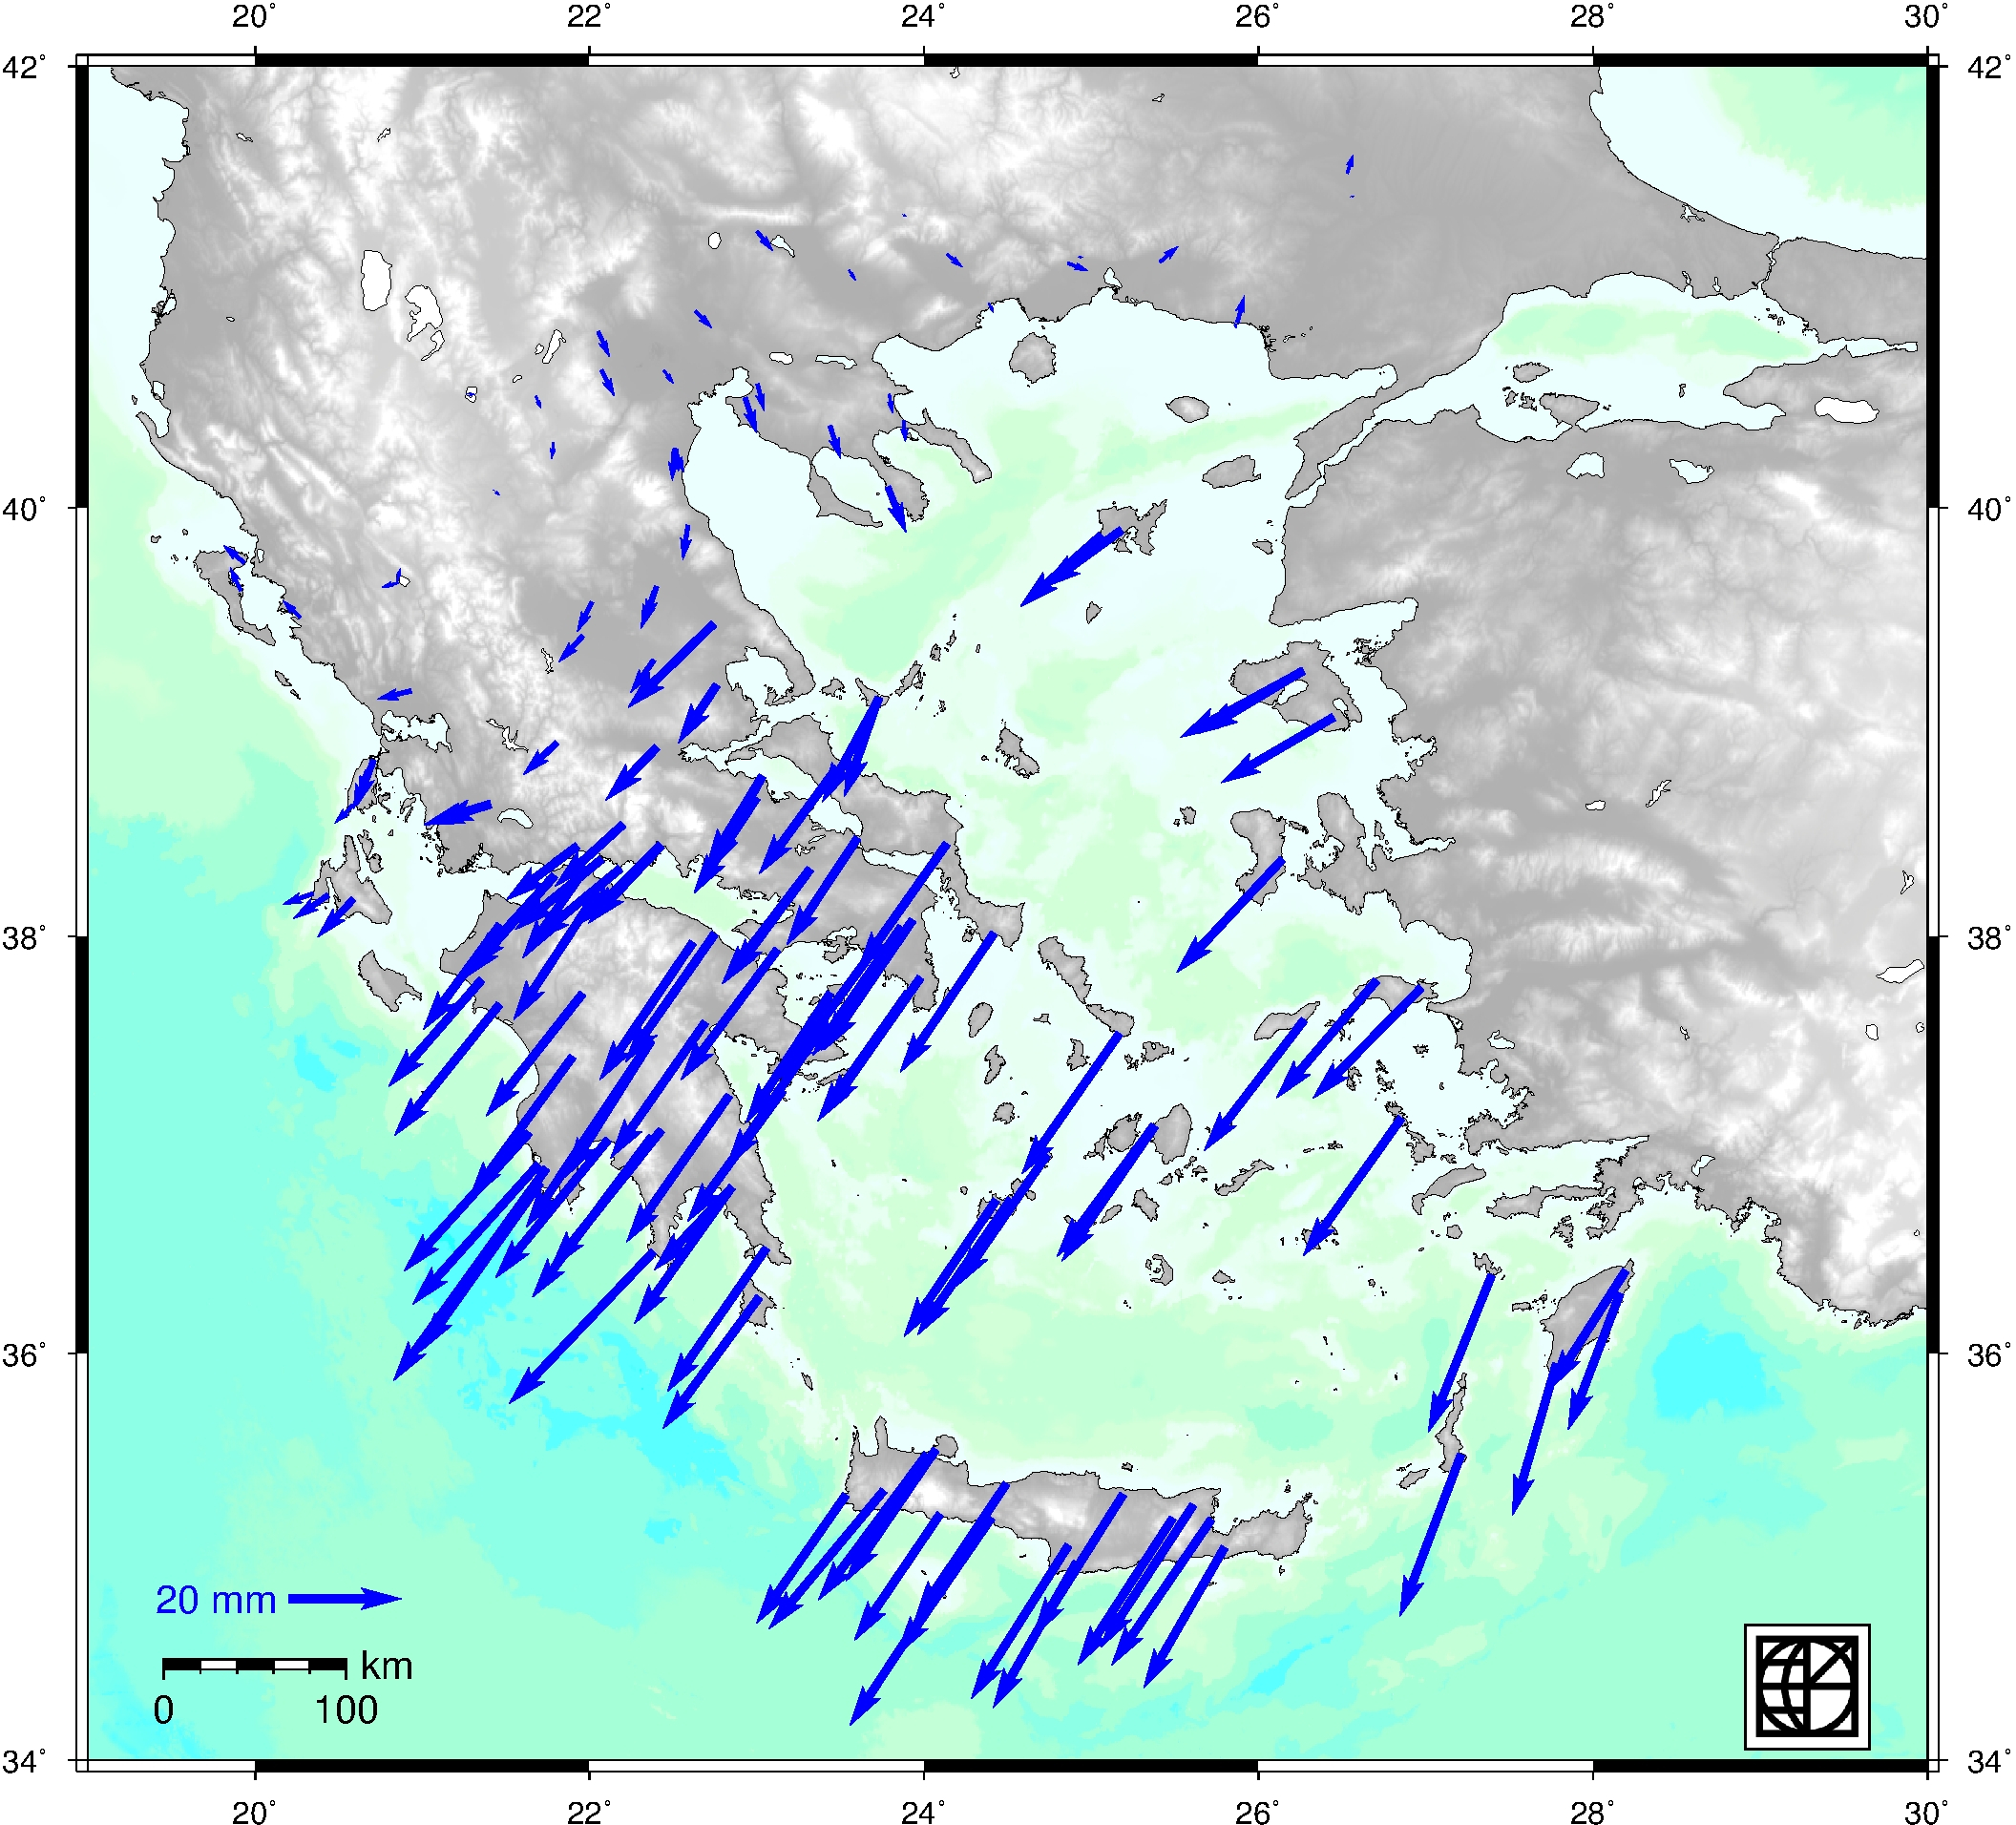
\includegraphics[width=.9\onecolwid]{testvel.jpg}
%     \caption{Tectonic velocities of all processed GNSS stations wrt fixed Europe.}
%     \label{fig:vels}
% \end{figure}
\end{block}

%----------------------------------------------------------------------------------------
%	REFERENCES
%----------------------------------------------------------------------------------------

\begin{block}{References}

\nocite{*} % Insert publications even if they are not cited in the poster
\footnotesize{\bibliographystyle{unsrt}
\bibliography{sample}\vspace{0.75in}}


\end{block}



%----------------------------------------------------------------------------------------

\end{column} % End of the third column

\end{columns} % End of all the columns in the poster

\end{frame} % End of the enclosing frame

\end{document}
